\section{Devices connection}

Due to the last two \direct features described in the previous section, devices cannot create and destroy connection opportunistically, so for our simulation we had to introduce a connection establishing phase which creates a \direct group and provides to all the devices a complete address map to let them communicate.
Devices connection setup consists of the following operations:
	\begin{itemize}
		\item One of the devices ask other devices for connection
		\item When a device accepts, it starts a DHCP negotiation with the connection starter. If no \direct group exists, a group is created and the starter device becomes the group owner; if requesting device is already an owner of a pre-existing group, the device is added to this group. At the end of this phase, each device has an IP address. Only group owner's IP is available via APIs. 
		\item Each device opens a TCP Server Socket on port 8888, listening for incoming connections.
		\item When a device connects to a group, it connects via Socket to the group owner sending a \emph{Ping message}. This message is used by the group owner to collect devices MAC/IP addresses: The first is included into the \emph{Ping message} by each device, the second indeed is obtained by the owner from the incoming Socket information (using Java APIs).
		\item After collecting all the couples \begin{center}\tt{<MAC address,IP address>}\end{center} from all the clients on a map, it sends it back to all the devices, to let them communicate directly.
	\end{itemize}
	
When all of this operations are done, all the devices are connected and can communicate each other directly via TCP Sockets. The created (overlay) network is visible in figure \ref{fig:device_network}

\begin{figure}[!htbp]
\centering
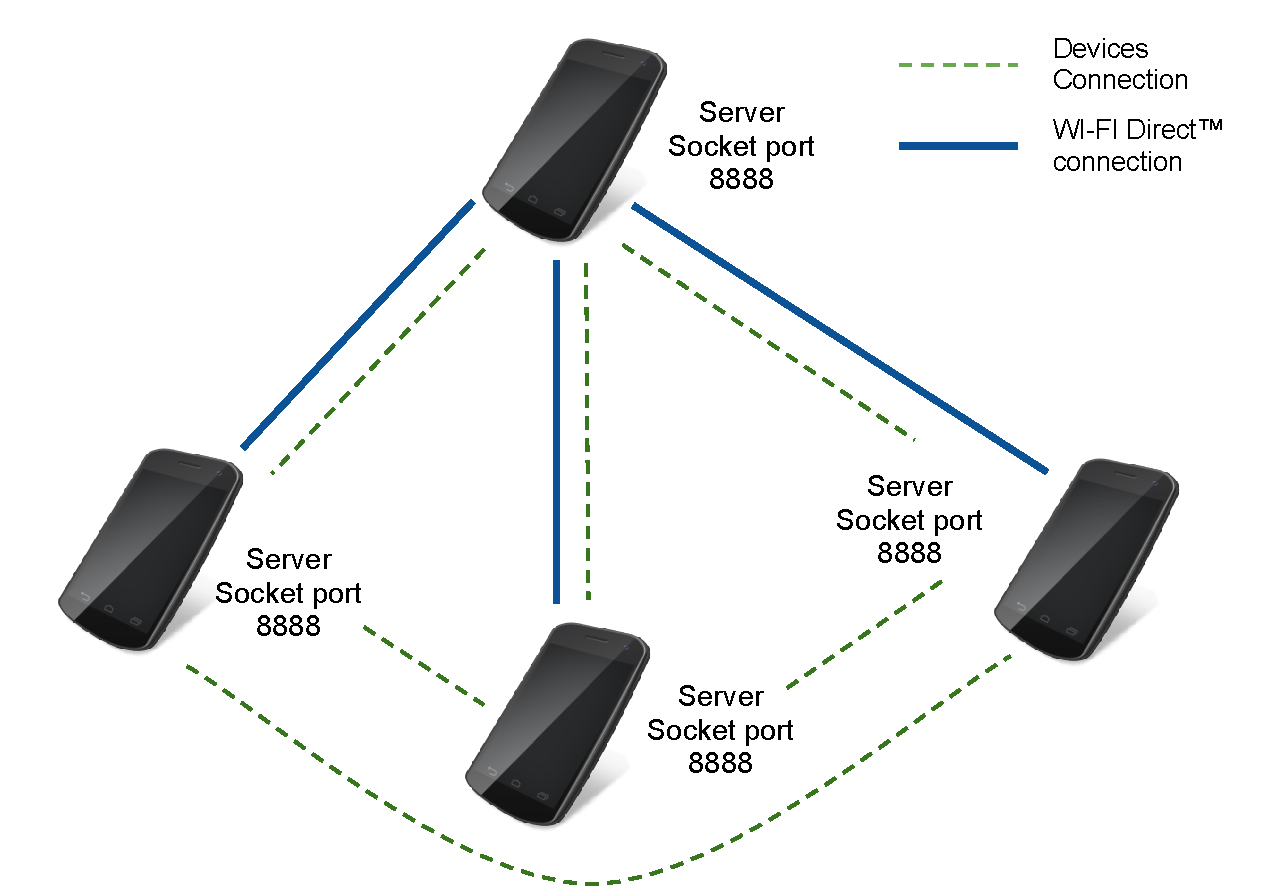
\includegraphics[width=3.6in]{imgs/Devices_network.pdf}
\caption{Devieces overlay network}
\label{fig:device_network}
\end{figure}
